% Problem 1
\section*{第1問　線形代数 \score{40}}
実数パラメータ $a$ に対して、行列
\[
A=\begin{pmatrix}
1 & a & 0\\
0 & 1 & 0\\
1 & 0 & 2
\end{pmatrix}
\]
を考える。以下の問いに答えよ。

\begin{enumerate}
  \item 特性多項式 $\det(\lambda I-A)$ を求め、$A$ の固有値をすべて求めよ。\score{8}
  \item 固有値 $\lambda=1$ および $\lambda=2$ に対する固有空間の基底を、$a=0$ と $a\neq 0$ の場合に注意して求めよ。\score{10}
  \item $A$ が対角化可能となるための $a$ の条件を求めよ。\score{6}
  \item 以下では $a=0$ とする。可逆行列 $P$ と対角行列 $D$ を一組求め、
  \[
  A=PDP^{-1}
  \]
  と表せ。\score{8}
  \item 自然数 $n$ に対して $A^n$ を求めよ。\score{8}
\end{enumerate}

\vfill
\begin{pointbox}
\textbf{答案上の注意：} 固有値の代数的重複度と固有空間の次元を区別して記述すること。
\end{pointbox}
\newpage

% Problem 2
\section*{第2問　多変数解析・重積分 \score{35}}
\begin{enumerate}
  \item 2変数関数
  \[
  f(x,y)=x^3+y^3-3xy
  \]
  について、停留点をすべて求め、それぞれが極大点・極小点・鞍点のいずれであるか判定せよ。必要に応じてヘッセ行列を用いてよい。\score{15}

  \item 領域
  \[
  D=\left\{(x,y)\in\R^2\mid 1\le x+y\le 2,\quad 0\le x-y\le 1\right\}
  \]
  に対して、重積分
  \[
  I=\iint_D (x^2-y^2)e^{x+y}\dd x\dd y
  \]
  を求めよ。変数変換
  \[
  u=x+y,\qquad v=x-y
  \]
  を用いてよい。\score{20}
\end{enumerate}

\vspace{6mm}
\begin{center}
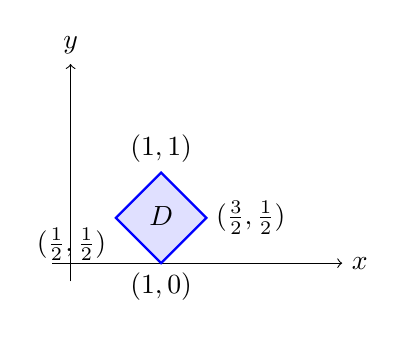
\begin{tikzpicture}[scale=1.15]
  \draw[->] (-0.2,0) -- (3.0,0) node[right] {$x$};
  \draw[->] (0,-0.2) -- (0,2.2) node[above] {$y$};
  \fill[Blue!12] (0.5,0.5)--(1,0)--(1.5,0.5)--(1,1)--cycle;
  \draw[Blue,thick] (0.5,0.5)--(1,0)--(1.5,0.5)--(1,1)--cycle;
  \node[below left] at (0.5,0.5) {$(\frac12,\frac12)$};
  \node[below] at (1,0) {$(1,0)$};
  \node[right] at (1.5,0.5) {$(\frac32,\frac12)$};
  \node[above] at (1,1) {$(1,1)$};
  \node at (1,0.52) {$D$};
\end{tikzpicture}
\end{center}
\newpage

% Problem 3
\section*{第3問　常微分方程式 \score{25}}
以下の初期値問題を解け。

\begin{enumerate}
  \item
  \[
  y'+2xy=x,\qquad y(0)=0.
  \]
  \score{10}

  \item
  \[
  y''-2y'+y=e^x,\qquad y(0)=0,\quad y'(0)=1.
  \]
  \score{15}
\end{enumerate}

\vspace{10mm}
\begin{pointbox}
\textbf{確認事項：}
1階方程式では積分因子を明示すること。2階方程式では右辺 $e^x$ が同次方程式の解と重なることに注意すること。
\end{pointbox}

\vfill
\begin{center}
\large\bfseries ここまでが問題編です。続いて解答用紙があります。
\end{center}
\newpage
